%%
%% Automatically generated file from DocOnce source
%% (https://github.com/hplgit/doconce/)
%%

% #define PREAMBLE

% #ifdef PREAMBLE
%-------------------- begin preamble ----------------------

\documentclass[%
oneside,                 % oneside: electronic viewing, twoside: printing
final,                   % draft: marks overfull hboxes, figures with paths
10pt]{article}

\listfiles               %  print all files needed to compile this document

\usepackage{relsize,makeidx,color,setspace,amsmath,amsfonts,amssymb}
\usepackage[table]{xcolor}
\usepackage{bm,ltablex,microtype}

\usepackage[pdftex]{graphicx}

\usepackage[T1]{fontenc}
%\usepackage[latin1]{inputenc}
\usepackage{ucs}
\usepackage[utf8x]{inputenc}

\usepackage{lmodern}         % Latin Modern fonts derived from Computer Modern

% Hyperlinks in PDF:
\definecolor{linkcolor}{rgb}{0,0,0.4}
\usepackage{hyperref}
\hypersetup{
    breaklinks=true,
    colorlinks=true,
    linkcolor=linkcolor,
    urlcolor=linkcolor,
    citecolor=black,
    filecolor=black,
    %filecolor=blue,
    pdfmenubar=true,
    pdftoolbar=true,
    bookmarksdepth=3   % Uncomment (and tweak) for PDF bookmarks with more levels than the TOC
    }
%\hyperbaseurl{}   % hyperlinks are relative to this root

\setcounter{tocdepth}{2}  % levels in table of contents

% Tricks for having figures close to where they are defined:
% 1. define less restrictive rules for where to put figures
\setcounter{topnumber}{2}
\setcounter{bottomnumber}{2}
\setcounter{totalnumber}{4}
\renewcommand{\topfraction}{0.95}
\renewcommand{\bottomfraction}{0.95}
\renewcommand{\textfraction}{0}
\renewcommand{\floatpagefraction}{0.75}
% floatpagefraction must always be less than topfraction!
% 2. ensure all figures are flushed before next section
\usepackage[section]{placeins}
% 3. enable begin{figure}[H] (often leads to ugly pagebreaks)
%\usepackage{float}\restylefloat{figure}

% --- fancyhdr package for fancy headers ---
\usepackage{fancyhdr}
\fancyhf{} % sets both header and footer to nothing
\renewcommand{\headrulewidth}{0pt}
\fancyfoot[LE,RO]{\thepage}
% Ensure copyright on titlepage (article style) and chapter pages (book style)
\fancypagestyle{plain}{
  \fancyhf{}
  \fancyfoot[C]{{\footnotesize \copyright\ 2018-2019, Christian Forssén. Released under CC Attribution-NonCommercial 4.0 license}}
%  \renewcommand{\footrulewidth}{0mm}
  \renewcommand{\headrulewidth}{0mm}
}
% Ensure copyright on titlepages with \thispagestyle{empty}
\fancypagestyle{empty}{
  \fancyhf{}
  \fancyfoot[C]{{\footnotesize \copyright\ 2018-2019, Christian Forssén. Released under CC Attribution-NonCommercial 4.0 license}}
  \renewcommand{\footrulewidth}{0mm}
  \renewcommand{\headrulewidth}{0mm}
}

\pagestyle{fancy}


\usepackage[framemethod=TikZ]{mdframed}

% --- begin definitions of admonition environments ---

% Admonition style "mdfbox" is an oval colored box based on mdframed
% "notice" admon
\definecolor{mdfbox_notice_background}{rgb}{1,1,1}
\newmdenv[
  skipabove=15pt,
  skipbelow=15pt,
  outerlinewidth=0,
  backgroundcolor=mdfbox_notice_background,
  linecolor=black,
  linewidth=2pt,       % frame thickness
  frametitlebackgroundcolor=mdfbox_notice_background,
  frametitlerule=true,
  frametitlefont=\normalfont\bfseries,
  shadow=false,        % frame shadow?
  shadowsize=11pt,
  leftmargin=0,
  rightmargin=0,
  roundcorner=5,
  needspace=0pt,
]{notice_mdfboxmdframed}

\newenvironment{notice_mdfboxadmon}[1][]{
\begin{notice_mdfboxmdframed}[frametitle=#1]
}
{
\end{notice_mdfboxmdframed}
}

% Admonition style "mdfbox" is an oval colored box based on mdframed
% "summary" admon
\definecolor{mdfbox_summary_background}{rgb}{1,1,1}
\newmdenv[
  skipabove=15pt,
  skipbelow=15pt,
  outerlinewidth=0,
  backgroundcolor=mdfbox_summary_background,
  linecolor=black,
  linewidth=2pt,       % frame thickness
  frametitlebackgroundcolor=mdfbox_summary_background,
  frametitlerule=true,
  frametitlefont=\normalfont\bfseries,
  shadow=false,        % frame shadow?
  shadowsize=11pt,
  leftmargin=0,
  rightmargin=0,
  roundcorner=5,
  needspace=0pt,
]{summary_mdfboxmdframed}

\newenvironment{summary_mdfboxadmon}[1][]{
\begin{summary_mdfboxmdframed}[frametitle=#1]
}
{
\end{summary_mdfboxmdframed}
}

% Admonition style "mdfbox" is an oval colored box based on mdframed
% "warning" admon
\definecolor{mdfbox_warning_background}{rgb}{1,1,1}
\newmdenv[
  skipabove=15pt,
  skipbelow=15pt,
  outerlinewidth=0,
  backgroundcolor=mdfbox_warning_background,
  linecolor=black,
  linewidth=2pt,       % frame thickness
  frametitlebackgroundcolor=mdfbox_warning_background,
  frametitlerule=true,
  frametitlefont=\normalfont\bfseries,
  shadow=false,        % frame shadow?
  shadowsize=11pt,
  leftmargin=0,
  rightmargin=0,
  roundcorner=5,
  needspace=0pt,
]{warning_mdfboxmdframed}

\newenvironment{warning_mdfboxadmon}[1][]{
\begin{warning_mdfboxmdframed}[frametitle=#1]
}
{
\end{warning_mdfboxmdframed}
}

% Admonition style "mdfbox" is an oval colored box based on mdframed
% "question" admon
\definecolor{mdfbox_question_background}{rgb}{1,1,1}
\newmdenv[
  skipabove=15pt,
  skipbelow=15pt,
  outerlinewidth=0,
  backgroundcolor=mdfbox_question_background,
  linecolor=black,
  linewidth=2pt,       % frame thickness
  frametitlebackgroundcolor=mdfbox_question_background,
  frametitlerule=true,
  frametitlefont=\normalfont\bfseries,
  shadow=false,        % frame shadow?
  shadowsize=11pt,
  leftmargin=0,
  rightmargin=0,
  roundcorner=5,
  needspace=0pt,
]{question_mdfboxmdframed}

\newenvironment{question_mdfboxadmon}[1][]{
\begin{question_mdfboxmdframed}[frametitle=#1]
}
{
\end{question_mdfboxmdframed}
}

% Admonition style "mdfbox" is an oval colored box based on mdframed
% "block" admon
\definecolor{mdfbox_block_background}{rgb}{1,1,1}
\newmdenv[
  skipabove=15pt,
  skipbelow=15pt,
  outerlinewidth=0,
  backgroundcolor=mdfbox_block_background,
  linecolor=black,
  linewidth=2pt,       % frame thickness
  frametitlebackgroundcolor=mdfbox_block_background,
  frametitlerule=true,
  frametitlefont=\normalfont\bfseries,
  shadow=false,        % frame shadow?
  shadowsize=11pt,
  leftmargin=0,
  rightmargin=0,
  roundcorner=5,
  needspace=0pt,
]{block_mdfboxmdframed}

\newenvironment{block_mdfboxadmon}[1][]{
\begin{block_mdfboxmdframed}[frametitle=#1]
}
{
\end{block_mdfboxmdframed}
}

% --- end of definitions of admonition environments ---

% prevent orhpans and widows
\clubpenalty = 10000
\widowpenalty = 10000

% --- end of standard preamble for documents ---


\usepackage[swedish]{babel}

\raggedbottom
\makeindex
\usepackage[totoc]{idxlayout}   % for index in the toc
\usepackage[nottoc]{tocbibind}  % for references/bibliography in the toc

%-------------------- end preamble ----------------------

\begin{document}

% matching end for #ifdef PREAMBLE
% #endif

\newcommand{\exercisesection}[1]{\subsection*{#1}}

\input{newcommands_keep}

% ------------------- main content ----------------------



% ----------------- title -------------------------

\thispagestyle{empty}

\begin{center}
{\LARGE\bf
\begin{spacing}{1.25}
Learning from data: Logistic Regression
\end{spacing}
}
\end{center}

% ----------------- author(s) -------------------------

\begin{center}
{\bf Christian Forssén${}^{1}$} \\ [0mm]
\end{center}


\begin{center}
{\bf Morten Hjorth-Jensen${}^{2, 3}$} \\ [0mm]
\end{center}

\begin{center}
% List of all institutions:
\centerline{{\small ${}^1$Department of Physics, Chalmers University of Technology, Sweden}}
\centerline{{\small ${}^2$Department of Physics, University of Oslo}}
\centerline{{\small ${}^3$Department of Physics and Astronomy and National Superconducting Cyclotron Laboratory, Michigan State University}}
\end{center}
    
% ----------------- end author(s) -------------------------

% --- begin date ---
\begin{center}
Oct 14, 2019
\end{center}
% --- end date ---

\vspace{1cm}


% !split 
\section{Logistic Regression}

In linear regression our main interest was centered on learning the
coefficients of a functional fit (say a polynomial) in order to be
able to predict the response of a continuous variable on some unseen
data. The fit to the continuous variable $y_i$ is based on some
independent variables $\boldsymbol{x}_i$. Linear regression resulted in
analytical expressions for standard ordinary Least Squares or Ridge
regression (in terms of matrices to invert) for several quantities,
ranging from the variance and thereby the confidence intervals of the
parameters $\boldsymbol{w}$ to the mean squared error. If we can invert
the product of the design matrices, linear regression gives then a
simple recipe for fitting our data.


Classification problems, however, are concerned with outcomes taking
the form of discrete variables (i.e.~categories). We may for example,
on the basis of DNA sequencing for a number of patients, like to find
out which mutations are important for a certain disease; or based on
scans of various patients' brains, figure out if there is a tumor or
not; or given a specific physical system, we'd like to identify its
state, say whether it is an ordered or disordered system (typical
situation in solid state physics); or classify the status of a
patient, whether she/he has a stroke or not and many other similar
situations.

The most common situation we encounter when we apply logistic
regression is that of two possible outcomes, normally denoted as a
binary outcome, true or false, positive or negative, success or
failure etc.

% !split
\subsection{Optimization and Deep learning}

Logistic regression will also serve as our stepping stone towards
neural network algorithms and supervised deep learning. For logistic
learning, the minimization of the cost function leads to a non-linear
equation in the parameters $\boldsymbol{w}$. The optimization of the
problem calls therefore for minimization algorithms. This forms the
bottle neck of all machine learning algorithms, namely how to find
reliable minima of a multi-variable function. This leads us to the
family of gradient descent methods. The latter are the working horses
of basically all modern machine learning algorithms.

We note also that many of the topics discussed here on logistic 
regression are also commonly used in modern supervised Deep Learning
models, as we will see later.


% !split 
\subsection{Basics and notation}

We consider the case where the dependent variables (also called the
responses, targets, or outcomes) are discrete and only take values
from $k=0,\dots,K-1$ (i.e.~$K$ classes).

The goal is to predict the
output classes from the design matrix $\boldsymbol{X}\in\mathbb{R}^{n\times p}$
made of $n$ samples, each of which carries $p$ features or predictors. The
primary goal is to identify the classes to which new unseen samples
belong.


\begin{notice_mdfboxadmon}[Notice]
We will use the following notation:
\begin{itemize}
\item $\boldsymbol{x}$: independent (input) variables, typically a vector of length $p$. A matrix of $n$ instances of input vectors is denoted $\boldsymbol{X}$, and is also known as the \emph{design matrix}.

\item $t$: dependent, response variable, also known as the target. For binary classification the target $t^{(i)} \in \{0,1\}$. For $K$ different classes we would have $t^{(i)} \in \{1, 2, \ldots, K\}$. A vector of $n$ targets from $n$ instances of data is denoted $\boldsymbol{t}$.

\item $\mathcal{D}$: is the data, where $\mathcal{D}^{(i)} = \{ (\boldsymbol{x}^{(i)}, t^{(i)} ) \}$.

\item $\boldsymbol{y}$: is the output of our classifier that will be used to quantify probabilities $p_{t=C}$ that the target belongs to class $C$.

\item $\boldsymbol{w}$: will be the parameters (weights) of our classification model.
\end{itemize}

\noindent
The subscript notation $y_i$ will here be used in parallel with the superscript one, $y^{(i)}$, for which the author apologizes.
\end{notice_mdfboxadmon} % title: Notice



Let us specialize to the case of two classes only, with outputs
$t_i=0$ and $t_i=1$. That is


\[
t_i = \begin{bmatrix} 0 \\  1 \end{bmatrix}
= \begin{bmatrix} \mathrm{no}\\  \mathrm{yes} \end{bmatrix}.
\]



% !split
\subsection{Linear classifier}

Before moving to the logistic model, let us try to use our linear
regression model to classify these two outcomes. We could for example
fit a linear model to the default case if $y_i > 0.5$ and the no
default case $y_i \leq 0.5$.

We would then have our 
weighted linear combination, namely 
\begin{equation}
\boldsymbol{\tilde{y}} = \boldsymbol{X}^T\boldsymbol{w} +  \boldsymbol{\epsilon},
\end{equation}
where $\boldsymbol{y}$ is a vector representing the possible outcomes, $\boldsymbol{X}$ is our
$n\times p$ design matrix and $\boldsymbol{w}$ represents our estimators/predictors.

% !split
\subsection{Some selected properties}

The main problem with our function is that it takes values on the
entire real axis. In the case of logistic regression, however, the
labels $t_i$ are discrete variables. 

One simple way to get a discrete output is to have sign
functions that map the output of a linear regressor to values $y_i \in \{ 0, 1 \}$,
$y_i = f(\tilde{y}_i)=\frac{sign(\tilde{y}_i)+1}{2}$, which will map to one if $\tilde{y}_i\ge 0$ and zero otherwise. 
We will encounter this model in our first demonstration of neural networks. Historically it is called the ``perceptron'' model in the machine learning
literature. This model is extremely simple. However, in many cases it is more
favorable to use a ``soft'' classifier that outputs
the probability of a given category. This leads us to the logistic function.


% !split
\subsection{The logistic function}

The perceptron is an example of a ``hard classification'' model. We
will encounter this model when we discuss neural networks as
well. Each datapoint is deterministically assigned to a category (i.e
$y_i=0$ or $y_i=1$). In many cases, it is favorable to have a ``soft''
classifier that outputs the probability of a given category rather
than a single value. For example, given $\boldsymbol{x}_i$, the classifier
outputs the probability of being in a category $k$.  Logistic regression
is the most common example of a so-called soft classifier. In logistic
regression, the probability that a data point $\boldsymbol{x}_i$
belongs to a category $t_i=\{0,1\}$ is given by the so-called logit function (or Sigmoid) which is meant to represent the likelihood for a given event, 
\[
y(\boldsymbol{x}; \boldsymbol{w}) = y(a) = \frac{1}{1+e^{-a}} = \frac{e^a}{1+e^a},
\]
where the so called \emph{activation} $a = a(\boldsymbol{x}; \boldsymbol{w})$. 

\begin{itemize}
\item Most frequently one uses $a = a(\boldsymbol{x}, \boldsymbol{w}) \equiv \boldsymbol{x} \cdot \boldsymbol{w}$.

\item Note that $1-y(a)= y(-a)$.

\item The sigmoid function can be motivated in several different ways. E.g.~in information theory this function represents the probability of a signal $s=1$ rather than $s=0$ when transmission occurs over a noisy channel.
\end{itemize}

\noindent
% !split
\subsection{Standard activation functions}


\begin{figure}[!ht]  % fig:logistic
  \centerline{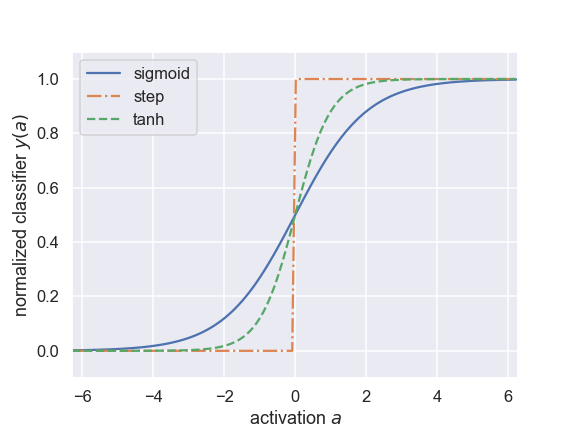
\includegraphics[width=0.8\linewidth]{fig/logistic_functions.png}}
  \caption{
  The sigmoid, step,and (normalized) tanh functions; three common classifier functions used in logistic regression and neural networks. \label{fig:logistic}
  }
\end{figure}
%\clearpage % flush figures fig:logistic


% !split
\subsection{A binary classifier with two parameters}

We assume now that we have two classes with $t_i$ either $0$ or $1$. Furthermore we assume also that we have only two parameters $w_0, w_1$ and the predictors $\boldsymbol{x}_i = \{ 1, x_i \}$ defining the Sigmoid function. We can produce probabilities from the classifier output $y_i$
\begin{align*}
p(t_i=1|x_i,\boldsymbol{w}) &= \frac{y(a_i)}{1 + y(a_i)} = \frac{\exp{(w_0+w_1x_i)}}{1+\exp{(w_0+w_1x_i)}},\nonumber\\
p(t_i=0|x_i,\boldsymbol{w}) &= 1 - p(t_i=1|x_i,\boldsymbol{w}) = \frac{1}{1 + y(a_i)} ,
\end{align*}
where $\boldsymbol{w} = \{ w_0, w_1\}$ are the weights we wish to extract from training data. 

% !split 
\paragraph{Maximum likelihood.}
In order to define the total likelihood for all possible outcomes from a  
dataset $\mathcal{D}=\{(x_i, t_i,)\}$, with the binary labels
$t_i\in\{0,1\}$ and where the data points are drawn independently, we use the binary version of the \href{{https://en.wikipedia.org/wiki/Maximum_likelihood_estimation}}{Maximum Likelihood Estimation} (MLE) principle. 
We express the 
likelihood in terms of the product of the individual probabilities of a specific outcome $t_i$, that is 
\begin{align*}
\mathcal{L} = P(\mathcal{D}|\boldsymbol{w})& = \prod_{i=1}^n \left[p(t_i=1|x_i,\boldsymbol{w})\right]^{t_i}\left[1-p(t_i=1|x_i,\boldsymbol{w}))\right]^{1-t_i}\nonumber \\
\end{align*}
from which we obtain the log-likelihood 
\[
L = \log(\mathcal{L}) = \sum_{i=1}^n \left( t_i\log{p(t_i=1|x_i,\boldsymbol{w})} + (1-t_i)\log\left[1-p(t_i=1|x_i,\boldsymbol{w}))\right]\right).
\]

The \textbf{cost/loss} function is then defined as the negative log-likelihood
\[
\mathcal{C}(\boldsymbol{w}) \equiv -L = -\sum_{i=1}^n \left( t_i\log{p(t_i=1|x_i,\boldsymbol{w})} + (1-t_i)\log\left[1-p(t_i=1|x_i,\boldsymbol{w}))\right]\right).
\]

% !split
\paragraph{The cost function rewritten as cross entropy.}
Using the definitions of the probabilities we can rewrite the \textbf{cost/loss} function as
\[
\mathcal{C}(\boldsymbol{w}) = -\sum_{i=1}^n \left( t_i\log{ y(x_i,\boldsymbol{w})} + (1-t_i)\log\left[ 1-y( x_i,\boldsymbol{w}) \right] \right),
\]
which can be recognised as the relative entropy between the empirical probability distribution $(t_i, 1-t_i)$ and the probability distribution predicted by the classifier $(y_i, 1-y_i)$.
Therefore, this cost function is known in statistics as the \textbf{cross entropy}. 

Using specifically the Sigmoid activation function with two weights, and reordering the logarithms, we can rewrite the log-likelihood as
\[
L(\boldsymbol{w}) = \sum_{i=1}^n  \left[ t_i(w_0+w_1 x_i) -\log{(1+\exp{(w_0+w_1x_i)})} \right].
\]

The maximum likelihood estimator is defined as the set of parameters (weights) that maximizes the log-likelihood (where we maximize with respect to $w$).

Since the cost (error) function is here defined as the negative log-likelihood, for logistic regression, we have that
\[
\mathcal{C}(\boldsymbol{w})=-\sum_{i=1}^n  \left[ t_i (w_0+w_1x_i) -\log{ \left( 1+\exp{(w_0+w_1x_i)} \right) } \right].
\]

% !split
\paragraph{Regularization.}
In practice, just as for linear regression, one often supplements the cross-entropy cost function with additional regularization terms, usually $L_1$ and $L_2$ regularization. This introduces hyperparameters into the classifier.

In particular, Lasso regularization is obtained by defining another cost function
\[
\mathcal{C}_W (\boldsymbol{w}) \equiv \mathcal{C} (\boldsymbol{w}) + \alpha E_W (\boldsymbol{w})
\]
where $E_W (\boldsymbol{w}) = \frac{1}{2} \sum_i w_i^2$ and $\alpha$ is known as the \emph{weight decay}.


\begin{question_mdfboxadmon}[Question]
Can you motivate why $\alpha$ is known as the weight decay? \emph{Hint}: Recall the origin of this regularizer from a Bayesian perspective.
\end{question_mdfboxadmon} % title: Question




% !split
\paragraph{Minimizing the cross entropy.}
The cross entropy is a convex function of the weights $\boldsymbol{w}$ and,
therefore, any local minimizer is a global minimizer. 


Minimizing this cost function (here without regularization term) with respect to the two parameters $w_0$ and $w_1$ we obtain

\begin{align*}
\frac{\partial \mathcal{C}(\boldsymbol{w})}{\partial w_0} 
&= -\sum_{i=1}^n  \left(t_i -\frac{\exp{(w_0+w_1x_i)}}{1+\exp{(w_0+w_1x_i)}}\right)
&= -\sum_{i=1}^n  \left(t_i - y_i \right), \\
\frac{\partial \mathcal{C}(\boldsymbol{w})}{\partial w_1} 
&= -\sum_{i=1}^n  \left(t_i x_i -x_i\frac{\exp{(w_0+w_1x_i)}}{1+\exp{(w_0+w_1x_i)}}\right)
&= -\sum_{i=1}^n  x_i \left(t_i - y_i \right).
\end{align*}

% !split
\paragraph{A more compact expression.}
Let us now define a vector $\boldsymbol{t}$ with $n$ elements $t_i$, an
$n\times 2$ matrix $\boldsymbol{X}$ which contains the $(1, x_i)$ predictor variables, and a
vector $\boldsymbol{y}$ of the outputs $y_i = y(x_i,\boldsymbol{w})$. We can then rewrite the first
derivative of cost function in matrix form

\[
\frac{\partial \mathcal{C}(\boldsymbol{w})}{\partial \boldsymbol{w}} = -\boldsymbol{X}^T\left( \boldsymbol{t}-\boldsymbol{y} \right). 
\]

% !split
\paragraph{A learning algorithm.}

\begin{notice_mdfboxadmon}[Notice]
Having access to the first derivative we can define an \emph{on-line learning rule} as follows:
\begin{itemize}
\item For each input $i$, compute the error $e_i = t_i - y_i$.

\item Adjust the weights in a direction that would reduce this error: $\Delta w_j = \eta e_i x_{j,i}$.

\item The parameter $\eta$ is called the \emph{learning rate}.
\end{itemize}

\noindent
This learning algorithm is a variant of \emph{stochastic learning}.
\end{notice_mdfboxadmon} % title: Notice



Alternatively, one can perform \emph{batch learning} for which multiple instances are combined into a batch, and the weights are adjusted following the matrix expression stated above. One can then repeat the training multiple times where each iteration consists of a \emph{forward pass} (computing the outputs $\boldsymbol{y}$ given a set of weights $\boldsymbol{w}$) and \emph{back-propagation} in which the gradient is computed and the weights are adjusted. At the end, one hopes to have reached an optimal set of weights.

% !split
\paragraph{Extending to more predictors.}
Within a binary classification problem, we can easily expand our model to include multiple predictors. Our activation function is then (with $p$ predictors)
\[
a( \boldsymbol{x}_i, \boldsymbol{w} ) = w_0 + w_1 x_{1,i} + w_2 x_{2,i} + \dots + w_p x_{p,i}.
\]
Defining $\boldsymbol{x}_i \equiv [1,x_{1,i}, x_{2,i}, \dots, x_{p,i}]$ and $\boldsymbol{w}=[w_0, w_1, \dots, w_p]$ we get
\[
p(t_i=1 | \boldsymbol{w}, \boldsymbol{x}_i) = \frac{ \exp{ \left( \boldsymbol{w} \cdot \boldsymbol{x}_i \right) }}{ 1 + \exp{ \left( \boldsymbol{w} \cdot \boldsymbol{x}_i \right) } }.
\]

% !split
\subsection{Including more classes}

Till now we have mainly focused on two classes, the so-called binary
system. Suppose we wish to extend to $K$ classes.  We will then need to have $K-1$ outputs $\boldsymbol{y}_i = \{ y_{1,i}, y_{2,i}, \ldots, y_{K-1,i} \}$. 


\begin{question_mdfboxadmon}[Question]
Why do we need only $K-1$ outputs if there are $K$ classes?
\end{question_mdfboxadmon} % title: Question



Let us for the sake of simplicity assume we have only two predictors. The activation functions for the outputs are (suppressing the index $i$)

\[
a_1 = w_{1,0}+w_{1,1}x_1,
\]

\[
a_2 = w_{2,0}+w_{2,1}x_1,
\]

and so on until the class $C=K-1$ class
\[
a_{K-1} = w_{(K-1),0}+w_{(K-1),1}x_1,
\]

and the model is specified in term of $K-1$ so-called log-odds or \textbf{logit} transformations $y_j = y(a_j)$.


% !split
\paragraph{Class probabilities: The Softmax function.}
The transformation of the multiple outputs, as described above, to probabilities for belonging to any of $K$ different classes is done via the so-called \textbf{Softmax} function.

The Softmax function is used in various multiclass classification
methods, such as multinomial logistic regression (also known as
softmax regression), multiclass linear discriminant analysis, naive
Bayes classifiers, and artificial neural networks.  Specifically, the predicted probability for the $k$-th class given a sample
vector $\boldsymbol{x}_i$ and a weighting vector $\boldsymbol{w}$ is (with two
predictors):

\[
p(t_i=k\vert \boldsymbol{x}_i,  \boldsymbol{w} ) = \frac{\exp{(w_{k,0}+w_{k,1}x_{1,i})}} {1+\sum_{l=1}^{K-1}\exp{(w_{l,0}+w_{l,1}x_{1,i})}}.
\]
It is easy to extend to more predictors. The probability for the final class is 
\[
p(t_i=K\vert \boldsymbol{x}_i,  \boldsymbol{w} ) = \frac{1} {1+\sum_{l=1}^{K-1}\exp{(w_{l,0}+w_{l,1}x_{1,i})}},
\]
which means that the discrete set of probabilities is properly normalized. 

Our earlier discussions were all specialized to
the case with two classes only. It is easy to see from the above that
what we derived earlier is compatible with these equations.

% ------------------- end of main content ---------------

% #ifdef PREAMBLE
\end{document}
% #endif

